\documentclass{article}
\usepackage[utf8]{inputenc}
\usepackage[english]{babel}
\usepackage{amsmath,amsfonts,amssymb,amsthm}
\usepackage{mathtools}
\usepackage{commath}
\usepackage[sc,osf]{mathpazo}
\usepackage{graphicx}
\usepackage{multicol}
\usepackage{tcolorbox}
\usepackage{rotating}
\usepackage{float}
\restylefloat{table}
\usepackage{subcaption}
\usepackage{placeins}
\usepackage[dvipsnames]{xcolor}
\usepackage[%  
    colorlinks=true,
    pdfborder={0 0 0},
    linkcolor=blue
]{hyperref}
\usepackage[colorinlistoftodos]{todonotes}
\usepackage{vmargin}  % Administrar márgenes
\setcounter{tocdepth}{3}
\setpapersize{A4} % Definir tamaño del papel
\setmargins{2.5cm} % Margen izquierdo
{1cm} % Margen superior
{16.5cm} % Área de impresión horizontal
{23.42cm} % Area de impresión vertical
{15mm} % Encabezado
{5mm} % Espacio entre el encabezado y el texto
{10pt} % Pie de página
{3mm} % Espacio entre el pie de página y el texto

\title{Repelling–Attracting Metropolis Algorithm^{~\ref{foot}}}
\author{Course Project under Prof. Dootika Vats}
\date{Submission Date: \today}

\begin{document}
\tableofcontents
\newpage
\maketitle

\section{Introduction and Overview}\footnote{\label{foot}Students: Anjan Kayal, Sunil Dhaka.}%overview is main here rather than intro of algo
In Monte Carlo Markov chain (MCMC) techniques the Metropolis Hastings is the most widely used and easy to implement algorithm. It is quite effective with low dimensional single mode distributions. It is not good in exploring multi model distributions. In this project we will present and implement the repelling attracting Metropolis (RAM) algorithm.
%full credit to the authors of paper%I don't feel like cutting anything here but still we should %write the same content in our own words after going through project once in writing 
%following lines are from abstract of the paper
The RAM
algorithm is a Metropolis-Hastings algorithm with a proposal that consists of a downhill move in density that
aims to make local modes repelling, followed by an uphill move in density that aims to make local modes
attracting. The downhill move is achieved via a reciprocal Metropolis ratio so that the algorithm prefers
downward movement. The uphill move does the opposite using the standard Metropolis ratio which prefers
upward movement. This down-up movement in density increases the probability of a proposed move to a
different mode. Because the acceptance probability of the proposal involves a ratio of intractable integrals,
we introduce an auxiliary variable which creates a term in the acceptance probability that cancels with the
intractable ratio. Using several examples, we demonstrate the potential for the RAM algorithm to explore a
multi modal distribution more efficiently than a Metropolis algorithm and with less tuning than is commonly
required by tempering-based methods.
\paragraph{}Through four numerical examples in later section of the project, we compare  RAM’s
performance to  commonly used Metropolis-Hastings algorithm. Our examples range from relatively
simple and high dimensional Gaussian mixtures (Examples 1
and 2) to lower dimensional, but more complex targets that arise
as posterior distributions in scientific problems (Examples 3 and
4). We compare RAM with standard Metropolis, implementing
both samplers with a common proposal distribution that is tuned to
improve the mixing of Metropolis for the particular multi modal
target distribution. These comparisons suggest that replacing
Metropolis with RAM when targeting a multi modal distribution
can be an efficient strategy, in terms of user’s effort. In our comparisons with tempering-based samplers, we find
that in moderate dimensions RAM performs as well as or better
than tempering-based methods, without the subtle tuning that
these methods require. We also show in Example 3 \& 4 how RAM can be embedded
within a Gibbs sampler to obtain satisfying results.  Because
RAM is able to jump between modes relatively often, it provides
good estimates of the relative size of the modes. In our examples, RAM obtains more reliable estimates of the mode sizes than
Metropolis. 
 
% Till this point 
% Task: come back to write from first page of paper after 2nd part done
\section{MH Algorithm}
We are going to review Metropolis Hastings algorithm to develop intuitions and to make connections with RAM algorithm, in later sections of paper. It will help us see how we are building RAM on top of Metropolis Hastings. After all, RAM is a MH algorithm with an unique joint proposal density.
\paragraph{}Suppose our target distribution from which we want to sample, is denoted by $F$. Here $F$ could be either normalized or unnormalized. It does not matter, we will see shortly. %tomorrow
On a continuous state space, Markov transition kernel can be denoted by $P(x,A)$ on $\mathbb{R}^k$. Basically, this transition kernel is a conditional probability distribution of a transition from any point $x \in \mathbb{R}^k$ to a point in a Borel set $A \in \mathcal{B}(\mathbb{R}^{k})$. Also notice that, since it is a distribution function,
$P(x,\mathbb{R}^{k}) = 1$, where it is permitted that the chain can make a transition from the point $x$ to $x$, i.e., $P(x, \{x\})$ is not necessarily zero. We assume that transition kernel is F-invariant, i.e., after large number of iterations, the distribution of the observations generated from the simulation is approximately the target distribution.%paper-need to be elaborated more
\paragraph{}Now, suppose we have the candidate-generating distribution or the proposal distribution. It is denoted by $Q(.,.)$. Given the current state $x$ the conditional density with respect to Lebesgue measure that generates a proposal $y$, is denoted by $q(x,y)$. The Markov transition kernel of MH is,$$P(x,A)=\int_{A} Q(x,dy)\alpha(x,y) + \delta_x(A) \int_{\chi} [1-\alpha(x,u)]Q(x,du).$$
Here first part corresponds to the transitions where $x \notequal y$ and the second part is the probability that process remains at $x$. The Hasting’s acceptance probability is defined as:
\begin{equation*}
\alpha(x,y)=min\left\{1,\frac{f(y)q(y,x)}{f(x)q(x,y)}\right\}
\end{equation*}
Notice that we do not need to know the target density with normalizing constant since both constants cancels out each other.
\paragraph{}Assuming all distributions are absolutely continuous with respect to the
Lebesgue measure, we can write the probability of moving away from $x$, that is, we accept proposal,
\begin{equation*}
A(x)=\int q(x,y)\alpha(x,y) dy.
\end{equation*}
Thus, we also can give the probability of staying at $x$,
\begin{equation*}
r(x)=1-A(x)=1-\int q(x,y)\alpha(x,y) dy.
\end{equation*}
If the proposal density is symmetric, i.e., $q(x,y)=q(y,x)$, then the MH reduces to Metropolis with acceptance probability as,
\begin{equation*}
\alpha(x,y)=min\left\{1,\frac{f(y)}{f(x)}\right\}.
\end{equation*}
\paragraph{}Basically, the Metropolis-Hastings MCMC algorithm proposes values from $Q(x,.)$ and then accepts or rejects them in a way that keeps $F$ invariant.
\begin{tcolorbox}[colback=blue!5!white,colframe=blue,title=Metropolis-Hastings Algorithm]
\begin{itemize}
\item Initialize with the (arbitrary) value $x^{(0)}$, and repeat for $i=1,2,\ldots,N$.
\item Generate proposal $y$ from $q(x^{(i-1)},.)$ and $u$ from $U(0,1)$, independently.
\item if $u \leq \alpha(x^{(i-1)},y)$, set $x^{(i)}=y$.
\item Otherwise, set $x^{(i)}=x^{(i-1)}$.
\item Return $\{x^{(1)},x^{(2)},\ldots,x^{(N)}\}$.
\end{itemize}
\end{tcolorbox}

\paragraph{}Metropolis is one of the most commonly used MCMC methods, but it often has difficulties exploring multi modal distributions, and tends to produce Markov chains that do not readily jump between local modes. There are alternative tempering methods to deal with multi modality  such as parallel tempering, simulated tempering , tempered transitions , and equi-energy sampler. %should we give these algorithms a little bit of explanations at least what they do in summary??
These methods usually require more tuning, which can be a constraint for practitioner.%tone of the paper needs to be changed - we are not creating it we are merely re-writing it with elaboration of some steps
Building on Metropolis, there is an alternative multi modal sampler called the repelling-attracting Metropolis
(RAM) algorithm, which is essentially as easy to implement as
the original Metropolis algorithm. RAM encourages a Markov
chain to jump between modes more frequently than Metropolis, and with less tuning requirements than tempering methods.
\section{RAM Algorithm}
We assume that $q$ is symmetric hereafter because RAM is currently feasible only with a symmetric $q$, that is, RAM can replace any Metropolis(symmetric MH) but not the more general MH algorithm. The main idea of RAM is a down-up jumping proposal density that generates a proposal $y$. To generate this proposal RAM consists of a forced downhill move in density via a reciprocal Metropolis ratio of the target densities in its acceptance probability that way the intermediate proposal prefers downward moves and makes local modes repelling, followed by an forced uphill move in density via a standard Metropolis ratio of the target densities in its acceptance probability that makes local modes attracting. We can draw from the down-up jumping proposal density but the MH acceptance probability for the joint proposal contains intractable integrals. We can avoid evaluating this ratio by introducing an auxiliary variable $z$. The resulting joint MH algorithm has an easily commutable acceptance ratio. Thus, RAM is a MH algorithm with an unique joint proposal density.
%make diagram-1
\begin{figure}[ht]
    \centering
    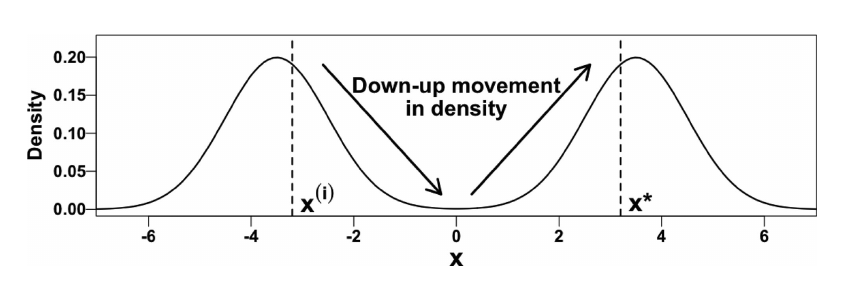
\includegraphics[width=\textwidth]{down-up.png}
    \caption{A repelling-attracting Metropolis algorithm is a Metropolis-Hastings algorithm that generates a proposal $x^{*}$ given the current state $x^{(i)}$ by making a down-up movement in density, that is, repelling–attracting to local modes, via forced downhill and uphill Metropolis transitions. The proposal $x^{*}$ has a higher chance to be near a mode other than the one of the current state, and it is then accepted or rejected in the usual way to preserve the stationary distribution.}
    \label{fig:downup}
\end{figure}
\subsection{Down-up Proposal}
We assume that all the densities are with respect to Lebesgue measure. 
\paragraph{}The down-up jumping proposal density, denoted by $q^{DU}(x,y)$, first generates an intermediate forced downhill proposal $y^{'}$ given the current state $x$, and then an forced uphill proposal $y$ given $y^{'}$. Hence, the down-up proposal density, $q^{DU}(x,y)$, by integrating out $y^{'}$:
\begin{equation*}
    q^{DU}(x,y)=\int q^U(y^{'},y) q^D(x,y^{'})dy^{'}
\end{equation*}
Here, $q^D$ and $q^U$ can be \textbf{any conditional density} functions with the property that they prefer lower and higher density states than the given states, respectively. We are choosing $q^D$ to be a forced downhill Metropolis kernel density. For any symmetric conditional density $q(.,.)$, we can define
a forced downhill Metropolis kernel density($q^D$) as
\begin{equation*}
    q^D(x,y^{'})=\frac{q(x,y^{'})\alpha_{\epsilon}^D(x,y^{'})}{\int q(x,y^{'})\alpha_{\epsilon}^D(x,y^{'})dy^{'}}.
\end{equation*}
Here,
\begin{equation*}
    \alpha_{\epsilon}^D(x,y^{'})=min\left\{1,\frac{(f(x)+\epsilon)q(x,y^{'})}{(f(y^{'})+\epsilon)q(y^{'},x)}\right\}=min\left\{1,\frac{f(x)+\epsilon}{f(y^{'})+\epsilon}\right\};\ \because{q(y^{'},x)=q(x,y^{'})}.
\end{equation*}
In above acceptance probability, $\epsilon$ is added. The reason is discussed below. We can write the normalizing constant, $$A^D(x)=\int q(x,y^{'})\alpha_{\epsilon}^D(x,y^{'})dy^{'}.$$
If $q$ is a proper density, that is, $\int q(x,y^{'})dy^{'} < \infty$, our normalizing constant $A^D(x)$ is finite because $0<\alpha_{\epsilon}^D(x,y^{'}) \leq 1$. We also have used term \textit{downhill} because we use reciprocal of standard Metropolis target density ratio in acceptance probability $\alpha_{\epsilon}^D(x,y^{'})$. Then, if the density $f(y^{'})$ is smaller than density $f(x)$, proposal $y^{'}$ gets accepted with probability one. Doing this it makes local modes repelling rather than attracting. 
\paragraph{}In similar fashion, we can define a forced uphill Metropolis transition kernel density($q^U$) as,
\begin{equation*}
    q^U(y^{'},y)=\frac{q(y^{'},y)\alpha_{\epsilon}^U(y^{'},y)}{\int q(y^{'},y)\alpha_{\epsilon}^U(y^{'},y)dy}.
\end{equation*}
Here,
\begin{equation*}
    \alpha_{\epsilon}^D(y^{'},y)=min\left\{1,\frac{(f(y)+\epsilon)q(y,y^{'})}{(f(y^{'})+\epsilon)q(y^{'},y)}\right\}=min\left\{1,\frac{f(y)+\epsilon}{f(y^{'})+\epsilon}\right\};\ \because q(y^{'},y)=q(y,y^{'}).
\end{equation*}
In above acceptance probability, $\epsilon$ is added for numerical stability since $f(y^{'})$ and $f(y)$ can be nearly zero when both $y^{'}$ and $y$ are in a valley between modes. Observe in figure ~\ref{fig:downup}. The value of $\epsilon$ may affect the convergence rate. To minimize its impact on the acceptance probability, we choose $\epsilon$ to be small with a default choice of $\epsilon$ to be machine precision number. \textbf{For symmetry}, we use $\epsilon$ in the same way in the acceptance probability of the downhill transition, $\alpha_{\epsilon}^D(x,y^{'})$.
We can write the normalizing constant, $$A^U(y^{'})=\int q(y^{'},y)\alpha_{\epsilon}^U(y^{'},y)dy.$$
If $q$ is a proper density, that is, $\int q(y^{'},y)dy < \infty$, our normalizing constant $A^U(y^{'})$ is finite because $0<\alpha_{\epsilon}^U(y^{'},y) \leq 1$. We also have used term \textit{uphill} because we use standard Metropolis target density ratio in acceptance probability $\alpha_{\epsilon}^D(y^{'},y)$. Then, if the density $f(y^{'})$ is smaller than density $f(y)$, proposal $y$ gets accepted with probability one. This kernel restores the attractiveness of local modes. 
\paragraph{}We have been using the term \textit{forced} because we are forcing it to accept a new value proposed through our kernel. We do it by repeatedly proposing values until it accepts one. As there is no possibility of staying at the same state, we don't have rejection probability term in Metropolis kernel density. Now, suppose we don't used forced kernel density, then the final proposal $y$ very well could be same as the current state $x$, when we get rejection in both the downhill and uphill Metropolis transitions, or $y$ could
be generated via only one of the downhill and uphill transitions if the other were rejected. This would not be helpful for
our purposes because it would not induce a down-up movement. Moreover, a forced transition kernel is mathematically
simpler than that of Metropolis since there only will be acceptance term.
\paragraph{}We have given $q^{DU}$ as,
\begin{equation*}
    q^{DU}(x,y)=\int q^U(y^{'},y) q^D(x,y^{'})dy^{'}.
\end{equation*}
It is clear that,
\begin{equation*}
    \int q^{DU}(x,y)dy=\int \int q^U(y^{'},y) q^D(x,y^{'})dy^{'}dy=1.
\end{equation*}
The \textbf{MH acceptance probability} with the down-up jumping density $q^{DU}$ simplifies to
\begin{equation*}
    \alpha^{DU}(x,y)=min\left\{1,\frac{f(y)q^{DU}(y,x))}{f(x)q^{DU}(x,y)}\right\}
\end{equation*}
We can get relation between $q^{DU}(x,y)$ and $q^{DU}(y,x)$, in following manner,
\begin{align*}
    q^{DU}(x,y)&=\int q^U(y^{'},y) q^D(x,y^{'})dy^{'}\\
    &=\int \frac{q(y^{'},y)\alpha_{\epsilon}^U(y^{'},y)}{A^U(y^{'})} \frac{q(x,y^{'})\alpha_{\epsilon}^D(x,y^{'})}{A^D(x)}dy^{'}\\
    q^{DU}(x,y)A^D(x)&=\int \frac{q(y^{'},y)\alpha_{\epsilon}^U(y^{'},y)}{A^U(y^{'})} q(x,y^{'})\alpha_{\epsilon}^D(x,y^{'})dy^{'}\\
    &=\int \frac{q(y,y^{'})\alpha_{\epsilon}^U(y^{'},y)}{A^U(y^{'})} q(y^{'},x)\alpha_{\epsilon}^D(x,y^{'})dy^{'}\\
\end{align*}
Placing $\alpha_{\epsilon}^U(y^{'},y)$ and $\alpha_{\epsilon}^D(x,y^{'})$, then rearranging them we get,
\begin{align*}
    q^{DU}(x,y)A^D(x)&=\int \frac{q(y,y^{'})\alpha_{\epsilon}^D(y,y^{'})}{A^U(y^{'})} q(y^{'},x)\alpha_{\epsilon}^U(y^{'},x)dy^{'}\\
    &=A^D(y)\int \frac{q(y,y^{'})\alpha_{\epsilon}^D(y,y^{'})}{A^D(y)} \frac{q(y^{'},x)\alpha_{\epsilon}^U(y^{'},x)}{A^U(y^{'})}dy^{'}\\
    &=q^{DU}(y,x)A^D(y).
\end{align*}
Hence, we can re-write MH acceptance probability as,
\begin{equation*}
    \alpha^{DU}(x,y)=min\left\{1,\frac{f(y)A^D(x))}{f(x)A^D(y)}\right\}.
\end{equation*}
% Anjan's part
\subsection{An Auxiliary Variable Approach}
Notice $\frac{A^{D}(x)}{A^{D}(y)}$ is an intractable  normalising constant in MH acceptance probability($\alpha^{DU}(x,y)$). One approach is to replace this ratio by an estimate calculated by Markov chain Monte Carlo methods, hoping that the algorithm then has an equilibrium distribution. We avoid such approximations. We will go for an auxiliary variable approach that avoids this ratio altogether. We form a joint Markov chain for $x$ and an auxiliary variable $z$ so that the target marginal density for $x$ is still $f$. Here $z$ is really of no interest when we run the Markov chain. It is just facilitating the running of the Markov chain and it would totally be ignored after we run the Markov chain. We set the joint target density as $f(x,z)=f(x)q(x,z)$. The acceptance probability of the joint proposal density,
\begin{equation*}
    \alpha^{J}((x,z^{'}),(y,z^{''}))= min\left\{1,\frac{f(y)min\left\{1,\frac{f(x)+\epsilon}{f(z^{'})+\epsilon}\right\}}{f(x)min\left\{1,\frac{f(y)+\epsilon}{f(z^{''})+\epsilon}\right\}}\right\}
\end{equation*}
\begin{proof}
Let us consider a generic joint target distribution $f(x,z)=f(x)g(x,z)$. Here $g(.,.)$ is any conditional distribution, at least for now. We will specify it later. We take a joint proposal density,
\begin{equation*}
    q^{J}((x,z^{'}),(y,z^{''})) = q_1((x,z^{'}),y)q_2((y,x,z^{'}),z^{''}) = q_1(x,y)q_2(y,z^{''})
\end{equation*}
Now The MH acceptance probability of the joint proposal density, carefully:)
\begin{equation*}
    \alpha^{J}((x,z^{'}),(y,z^{''}))=min\left\{1,\frac{(f(y)g(y,z^{''})q_1(y,x)q_2(x,z^{'}))}{(f(x)g(x,z^{'})q_1(x,y)q_2(y,z^{''}))}\right\}
\end{equation*}
Notice that it is the proposal densities that are intractable here. It could be the case that we are able to sample from $q_1$, but are not able to evaluate $q_1$, due to unknown normalizing constant. We can find a function $h(.)$ such that $\frac{q_1(y,x)}{q_1(x,y)}=\frac{h(x)}{h(y)}$ because  the ratio of two (compatible) conditional densities equals the corresponding ratio of marginal densities, where $h$ itself may or may not be possible to evaluate. Now questions is how can we get ride of this ratio? If we can find a function $q_2$ such that its normalizing constant is proportional to $h$, then ratios cancel out each other. This way the joint acceptance probability becomes free of the intractable quantities.
\paragraph{}For this proposed RAM algorithm, we choose, $q_1(x,y)=q^{DU}(x,y)$. Then using result from Down-UP proposal section we have $\frac{h(x)}{h(y)}=\frac{A^D(x)}{A^D(y)}$. Now recall that downhill MKD is propositional to $A^D(.)$. So for eliminating these intractable normalizing constants, we choose $q_2(y,z^{''})=q^{D}(y,z^{''})$. Following the paper we choose $g(.,.)$ to be same as $q(.,.)$. So $g(y,z^{''})=q(y,z^{''})$. Now we can simplify,
\begin{align*}
    \alpha^{J}((x,z^{'}),(y,z^{''}))&=min\left\{1,\frac{(f(y)q(y,z^{''})q^{DU}(y,x)q^D(x,z^{'}))}{(f(x)q(x,z^{'})q^{DU}(x,y)q^D(y,z^{''}))}\right\}\\
    &=min\left\{1,\frac{f(y)q(y,z^{''})A^D(x)q(x,z^{'})\alpha_{\epsilon}^D(x,z^{'})A^D(y)}{f(x)q(x,z^{'})A^D(y)q(y,z^{''})\alpha_{\epsilon}^D(y,z^{''})A^D(x)}\right\}\\
    &=min\left\{1,\frac{f(y)\alpha_\epsilon^{D}(z^{'},x)}{f(x)\alpha_\epsilon^{D}(z^{''},y)}\right\}\\
    &= min\left\{1,\frac{f(y)min\left\{1,\frac{f(x)+\epsilon}{f(z^{'})+\epsilon}\right\}}{f(x)min\left\{1,\frac{f(y)+\epsilon}{f(z^{''})+\epsilon}\right\}}\right\}
\end{align*}
\end{proof}
\paragraph{Remark:}As a special case we can find that $f(z^{''})$ is likely to be smaller than $f(y)$ since $z^{''}$ is generated by the forced downhill transition and $f(z^{'})$ is likely to be smaller than $f(x)$ since $z^{'}$ is generated by the forced downhill transition. Then minimum of both quantities is 1. So the joint acceptance probability reduces to the acceptance probability of Metropolis algorithm.

\subsection{Implementation of the RAM Algorithm}
Now after finishing all the steps individually, we write the RAM algorithm in one place. In each RAM iteration, meaning to generate one sample, we need to go through four steps, outlines in Algorithm box. The first three generate a joint proposal, $(y,z^{''})$, via three consecutive forced transitions. The fourth step determines if the joint proposal is accepted or not, using the joint acceptance probability ratio.
\begin{tcolorbox}[colback=blue!5!white,colframe=blue,title=Repelling–Attracting Metropolis Algorithm]
\begin{itemize}
    \item \texttt{Initialization:} Set value for $x_0$ and $z_0^{'}=x_0$. To update for i=0,1,2,\ldots
    \item \texttt{Step-1(Downhill):} Repeatedly sample $y^{'} \sim q(x_i,y^{'})$ \& $U_1 \sim Uniform(0,1)$ until $$U_1 < min\left\{1,\frac{f(x_i)+\epsilon}{f(y^{'})+\epsilon}\right\}$$.
    \item \texttt{Step-2(Uphill):} Repeatedly sample $y \sim q(y^{'},y)$ \& $U_2 \sim Uniform(0,1)$ until $$U_2 < min\left\{1,\frac{f(y)+\epsilon}{f(y^{'})+\epsilon}\right\}$$
    \item \texttt{Step-3(Downhill):} Repeatedly sample $z^{''} \sim q(y,z^{''})$ \& $U_3 \sim Uniform(0,1)$ until $$U_3 < min\left\{1,\frac{f(y)+\epsilon}{f(z^{''})+\epsilon}\right\}$$
    \item \texttt{Step-4(Accept-Reject):} Sample $U_4 \sim Uniform(0,1)$, Set $(x_{i+1},z_{i+1}^{'})=(y,z^{''})$, $$\text{If  } U_4 < min\left\{1,\frac{f(y)min\left\{1,\frac{f(x_i)+\epsilon}{f(z_i^{'})+\epsilon}\right\}}{f(x_i)min\left\{1,\frac{f(y)+\epsilon}{f(z^{''})+\epsilon}\right\}}\right\}$$
    Otherwise, Set $(x_{i+1},z_{i+1}^{'})=(x_i,z_i^{'})$.
\end{itemize}
\end{tcolorbox}
\clearpage
\section{Numerical Examples}
\subsection{Example 1: A Mixture of Twenty Bivariate Gaussian
Densities
}
To compare the RAM with other algorithms, we are going to consider sampling from a two-dimensional normal mixture distribution,
%why the paper has written \sigma_i^2 rather than \sigma_i
\begin{equation*}
    f(x)=\frac{1}{2\pi}\sum_{i=1}^N \frac{w_i}{\sigma_i^2} exp\left\{-\frac{1}{2 \sigma_i^2}(x-\mu_i)^\top I_2 (x-\mu_i)\right\}
\end{equation*}
Here $x=(x_1,x_2)^\top$ and we take co variance matrix to be simply $\sigma_i^2 I_2$. For easy interpretations and to understand better, we consider $N=20$. The mean vectors $\{\mu_1,\ldots,\mu_{20}\}$ are uniformly drawn from the rectangle [0,10] x [0,10]. Look at the code for numbers. These numbers have been taken same as Kou, Zhou, and Wong (2006). This is being done just that we can compare RAM to the equi-energy sampler(EES) and parallel tempering(PT) from Kou, Zhou, and Wong (2006). Though, we will implement RAM code as general as possible so that RAM can be done for any mean vectors sample from the rectangle. Notice, that most local modes are more than 15 standard deviations away from the nearest ones, this mixture distribution poses a serious challenge for sampling algorithms, and thus serves as a good test. These are observable in figure ~\ref{fig:exa1.1}. Now, we take into account variances($\sigma_i$'s) \& weights($w_i$'s) under two different cases to specify our target distribution.
\begin{figure}[ht]
    \centering
    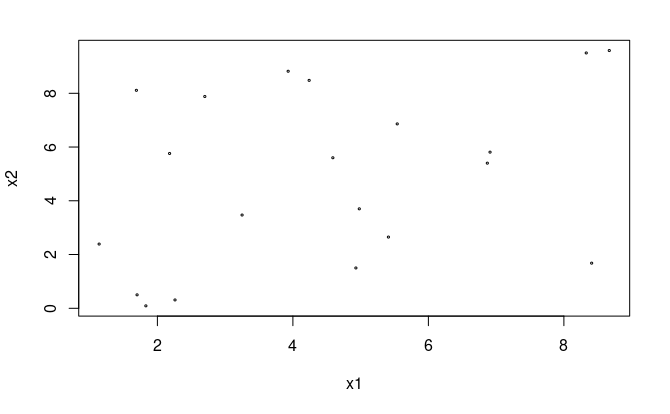
\includegraphics[width=\textwidth]{1.png}
    \caption{Point plot of modes for a mixture of 20 bivariate Gaussian densities}
    \label{fig:exa1.1}
\end{figure}
\paragraph{Case-a}
For this, we consider when all modes are equally weighted and have equal variances. For specific value of $\sigma_i$'s, we follow from Kou, Zhou, and Wong (2006),
\begin{align*}
    \sigma_1=\ldots=\sigma_{20}=0.1\\
    w_1=\ldots=w_{20}=0.05.
\end{align*}
Again, note that these values are just that we can compare RAM with other algorithms. Contour plot of this target distribution is given below(~\ref{fig:exa1.2}).
%fig:

\paragraph{Case-b}
In this case we consider all weights and variances are unequal for each component. They depend on Euclidean norm distance($d_i$) of their modes($\mu_i$) from the center $(5,5)$, such that, higher weight is given to modes that are near to (5,5) and such modes also have lower variances. Thus, weights and variances are defined as,
\begin{align*}
    \sigma_i^2 &=\frac{d_i}{20}\\
    w_i &=\frac{1}{d_i}.
\end{align*}
Here $d_i=\norm{\mu_i -(5,5)^\top}$. Contour plot of this target distribution is given above(~\ref{fig:exa1.2}).
%fig:
\begin{figure}
    \centering
    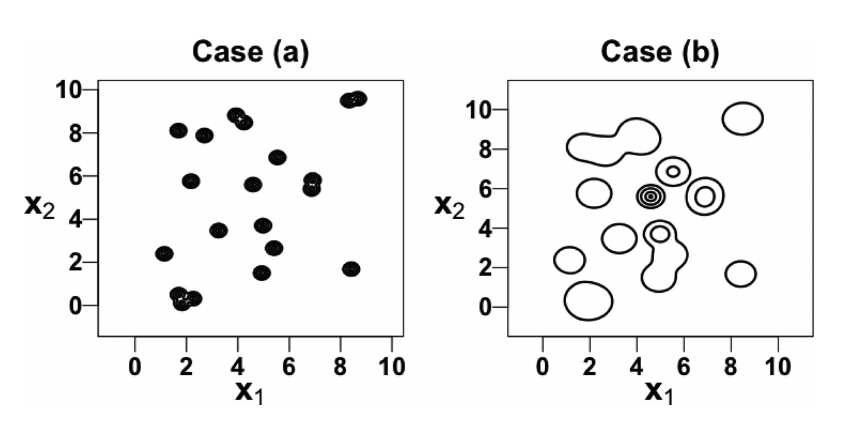
\includegraphics[width=\textwidth]{exa-1-point-plot.png}
    \caption{The first panel exhibits the contour plot of the target density in Example 1,
case (a) and the second panel shows that of the target density in Example 1, case (b).
The plotted contours outline regions with probability 1\%, 10\%, 50\%, and 95\% under
$f (x)$.
}
    \label{fig:exa1.2}
\end{figure}
\paragraph{Proposal Distribution:}We set the proposal distribution $q$ to be Gaussian with co-variance matrix $\sigma^2 I_2$, where $I_2$ is the identity matrix of dimension 2. To tune $\sigma$ , we initialize ten independent chains with 10 different values of $\sigma \in \{3.0, 3.5, \ldots, 7.5\}.$ %do we need to code it
Following Kou, Zhou, and Wong (2006), we set $\sigma$ to the
value that leads to \textbf{the best auto correlation} function among
those that visit all modes. This is 4.0 in case (a) and 3.5 in
case (b). These numbers have been taken from the paper. For both cases the chain is initialized at random values $x=x^{(0)}$ \& $z^{'}=z^{(0)}$ in the unit square, [0,1] x [0,1]. We choose one-third/one-fourth of the iterations/samples as burn-in.
\paragraph{Results:}First, we compare the average evaluation cost of each algorithm. To do that we report(in code), the expected total number of evaluations of
the target density $f$ needed to obtain the final sample, including burn-in, divided by the final sample size. We define four numbers:
\begin{itemize}
    \item $N_\pi$ = the average number of target density
evaluations at each iteration; 
\item $N_d$ = the average number of downhill proposals for RAM; \item $N_u$ = the average number of uphill proposals for RAM; \item $N_z$ = the average number
of downhill proposals for the auxiliary variable for RAM.
\end{itemize}
We notice that the average number of downhill proposals for intermediary variable($y^{'}$) and auxiliary variable, it is around 1, meaning, the
downhill proposals are usually accepted on the
first try. However, the number of proposals needed for the uphill
move in Step 2 varies. Generating a higher density proposal becomes challenging, and
the uphill transition in Step 2 requires more proposals. Hence, to know overall situation it suffices to only look at $N_\pi$. From the appendix of the paper we have, $N_\pi^{EE}=16$ \& $N_\pi^{PT}=16$. For RAM, $N_\pi^{RAM}=6.955$ in case (a) and $N_\pi^{RAM}=4.948$ in case (b). Notice that more evaluations are needed in case (a) than it is in case (b). The reason is the area of near zero density is
much larger than that in case (b). It can be noticed in figure ~\ref{fig:exa1.2}. Now in forced uphill step we require more proposal until it gets accepted, so it implies we need more evaluation of the target density.
\paragraph{}Due to computational costs we have only run the RAM algorithm for 10,000 total iterations, and initial 2500 iterations have been taken as burn-in. It is obvious that with more iterations we get more reliable data. Note that we have used the data given in the paper only for such comparison and conclusions. Due to low iterations our data is not a true representation of the RAM algorithm. We believe with increase in iterations we will reach the data given in the paper. To compare the accuracy of the moment estimates obtained
with the algorithms, we follow Kou, Zhou, and Wong
(2006) and run 20 independent chains using RAM. Table 1 summarizes the comparisons, where the ratios of the mean squared
error (MSE) of both EE and PT to that of RAM are all greater
than one. The improvement is particularly striking for case (b).
These indicate that RAM leads to a more reliable proportion of
iterations that are associated with each mode across the 20 runs.

\begin{table}[H]
\caption{Moment estimates for cases (a) and (b) based on 20 independent chains, each of length 10,000 generated with RAM, EE (equi-energy sampler), and PT (parallel
tempering). The results for EE and PT are from Kou, Zhou, and Wong (2006), and presented in their original format: Sample average (sample standard deviation) over the
20 replications.} % title of Table
\centering % used for centering table
\begin{tabular}{c c c c c c c} % centered columns (4 columns)
\hline\hline %inserts double horizontal lines
Case-(a) & Truth & RAM & EE & PT & \small{MSE(EE/RAM)} & \small{MSE(PT/RAM)} \\ [0.5ex] % inserts table
%heading
\hline % inserts single horizontal line
$E(x_1)$ & 4.478 & 4.5563(0.091) & 4.5019(0.170) & 4.4185(0.170) & 1.44 & 3.89 \\ [1ex]% inserting body of the table
$E(x_2)$ & 4.905 & 4.8000(0.101) & 4.9439(0.139) & 4.8790(0.283) & 1.91 & 7.40 \\[1ex]
$E(x_1^2)$ & 25.605 & 26.3734(0.900) & 25.9241(1.098) & 24.9856(1.713) & 1.61 &4.09 \\[1ex]
$E(x_2^2)$ & 33.920 & 32.7600(1.100) & 34.4763(1.373) & 33.5966(2.867) & 1.69 & 6.39 \\[1ex] % [1ex] adds vertical space
\hline %inserts single line
Case-(b) & Truth & RAM & EE & PT & \small{MSE(EE/RAM)} & \small{MSE(PT/RAM)} \\ [0.5ex] % inserts table
%heading
\hline % inserts single horizontal line
$E(x_1)$ & 4.688 & 4.6338(0.026) & 4.699(0.072) & 4.709(0.116) & 5.89 & 15.42 \\ [1ex]% inserting body of the table
$E(x_2)$ & 5.030 & 4.9956(0.035) & 5.037(0.086) & 5.001(0.134) & 6.07 & 15.33 \\[1ex]
$E(x_1^2)$ & 25.558 & 25.3694(0.263) & 25.693(0.739) & 25.813(1.122) & 7.87 &18.47 \\[1ex]
$E(x_2^2)$ & 31.378 & 31.5031(0.334) & 31.433(0.839) & 31.105(1.186) & 6.01 & 12.59 \\[1ex] % [1
\end{tabular}
\label{table:nonlin} % is used to refer this table in the text
\end{table}
\begin{figure}[ht]
\begin{subfigure}{.5\textwidth}
  \centering
  % include first image
  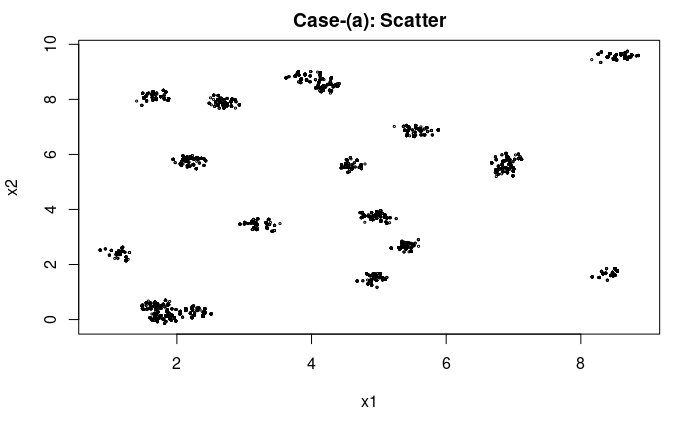
\includegraphics[width=.8\linewidth]{a1.png}  
  %\caption{Put your sub-caption here}
  \label{fig:sub-first}
\end{subfigure}
\begin{subfigure}{.5\textwidth}
  \centering
  % include second image
  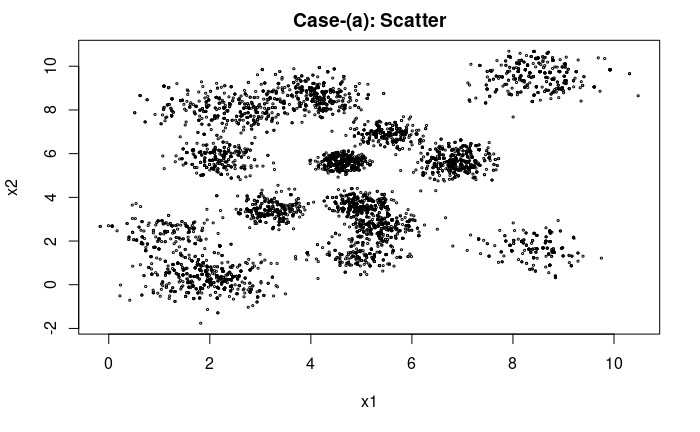
\includegraphics[width=.8\linewidth]{b1.png}  
  %\caption{Put your sub-caption here}
  \label{fig:sub-second}
\end{subfigure}
\caption{Bivariate Scatter plots}
\label{fig:fig}
\end{figure}
\begin{figure}[ht]
\begin{subfigure}{.5\textwidth}
  \centering
  % include first image
  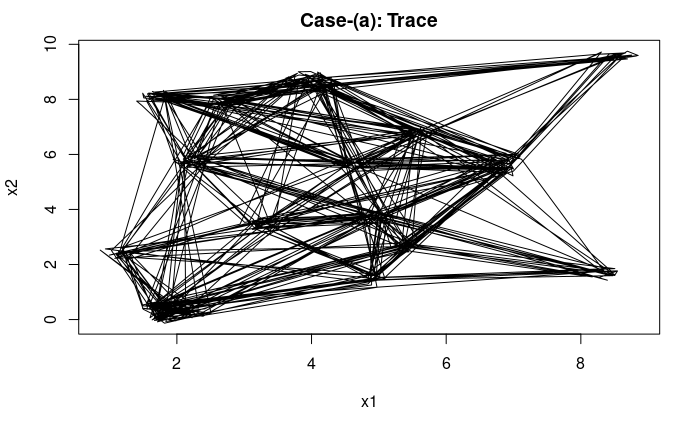
\includegraphics[width=.8\linewidth]{a2.png}  
  %\caption{Put your sub-caption here}
  \label{fig:sub-first}
\end{subfigure}
\begin{subfigure}{.5\textwidth}
  \centering
  % include second image
  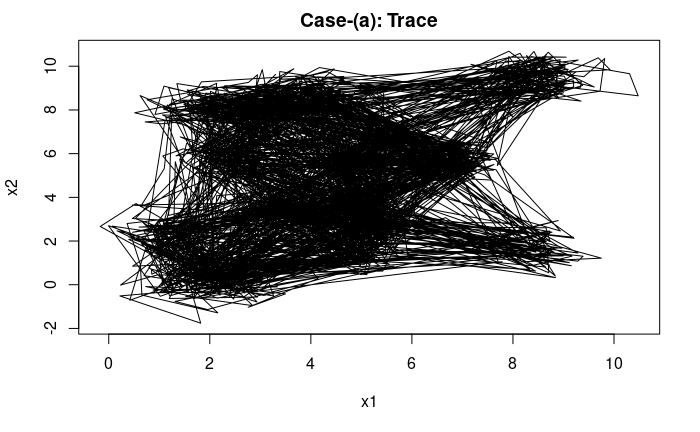
\includegraphics[width=.8\linewidth]{b2.png}  
  %\caption{Put your sub-caption here}
  \label{fig:sub-second}
\end{subfigure}
\caption{Bivariate Trace Plots}
\label{fig:fig}
\end{figure}
\begin{figure}[ht]
\begin{subfigure}{.5\textwidth}
  \centering
  % include first image
  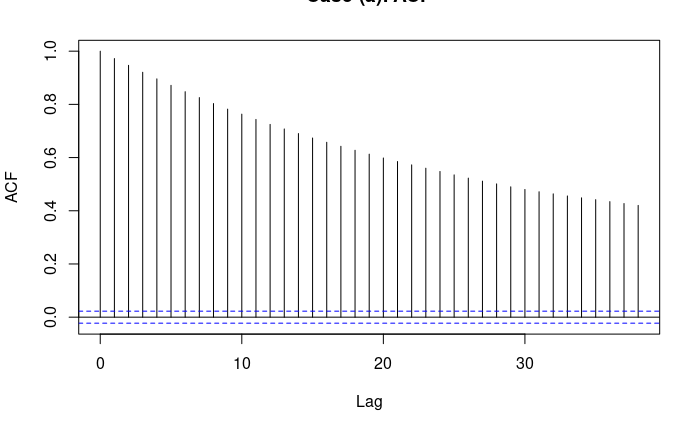
\includegraphics[width=.8\linewidth]{a3.png}  
  \caption{Case-a}
  \label{fig:sub-first}
\end{subfigure}
\begin{subfigure}{.5\textwidth}
  \centering
  % include second image
  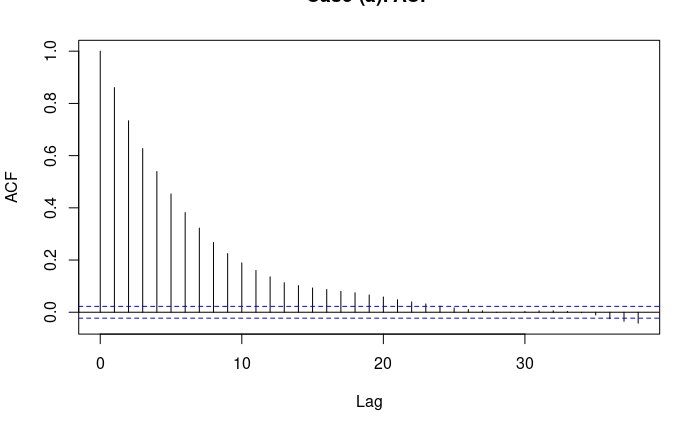
\includegraphics[width=.8\linewidth]{b3.png}  
  \caption{Case-b}
  \label{fig:sub-second}
\end{subfigure}
\caption{ACF Plots}
\label{fig:fig}
\end{figure}

\subsection{Example 2: High-Dimensional Multimodal
Distributions
}
For this example we are going to consider a equal mixture of  d-dimensional Gaussian distributions with $\mathbf{\Sigma}=I_d$. Following the paper we choose number of Gaussian($k$)$=8$. So we can write,
\begin{equation*}
    f(\mathbf{x}) \propto \sum_{k=1}^8 exp\left(-\frac{1}{2}(\mathbf{x}-\mu_k)^\top(\mathbf{x}-\mu_k)\right),
\end{equation*}
here $\mathbf{x}$ is an d-dimensional vector, that means, $\mathbf{x}=[x_1,\ldots,x_d]^\top$. Now to specify our target distribution, we follow the paper. In the paper the eight mean vectors are
defined by setting their first three coordinates(minimum of $d>2$) to the eight vertices of a cube of edge length 10 situated with its corner at the
origin and their remaining coordinates are filled with (10, 0) or
(0, 10) repeatedly. Please look code for numbers.
As paper have done to go with $d \in \{3,5,7,9,11\}$, we also do this for same dimensions. It can be done with any d-dimension. We do for only these $d$'s, so that we can compare with other algorithms. We also assume that the first two modes $\mu_1$ \& $\mu_2$ are known, perhaps
from an initial search, while the other six modes are unknown.
\paragraph{Proposal Distribution:}For simplicity, we use Gaussian jumping rules, though any
symmetric density can be used. Specifically, we consider a
d-dimensional Gaussian density with covariance matrix $\mathbf{\Sigma_q}$; both RAM and Metropolis share the same tuning parameter $\mathbf{\Sigma_q}$. RAM is designed to improve the ability of
Metropolis to jump between modes using a jumping rule that is
tuned to optimize Metropolis for the multimodal target. So, we set proposal distribution $q$ to be a d-dimensional Gaussian density with co-variance matrix $\mathbf{\Sigma_q}$. To achieve a reasonable acceptance rate, we first
run two Metropolis chains each of length 5000, initialized at the
two known mode locations and using a Gaussian jumping rule
with co-variance matrix $(\frac{2.382}{d})I_d$ , where $I_d$ is the identity
matrix. We then set $\mathbf{\Sigma_q}$ to the sample covariance matrix of the
combined sample from the two chains. To improve Metropolis’ ability to jump between modes, we reset $\mathbf{\Sigma_q}$ to the sample
covariance matrix of the burn-in sample. This one-time adaptation does not affect the validity of the resulting chain.  One could do still better with additional tuning of RAM.
For example, if $\mathbf{\Sigma_q}$ is tuned to optimize Metropolis for a multi-
modal target, we can simply set the covariance matrix of q for
RAM to $\mathbf{\Sigma_q}$/2 because RAM’s down-up proposal is generated by
two (down-up) Metropolis transitions. 
\paragraph{Results:}For each $d$, we run RAM ten times to obtain ten chains each
of length 10,000, discarding the first 2500 iterations of each
chain as burn-in. RAM’s average evaluation cost $N_\pi^{RAM}$
 is increases with increase in $d$. Also not that $N_u$,that is, the average number of uphill proposals for RAM, is the main component of $N_\pi^{RAM}$ that grows. $N_d$ \& $N_z$ are more or less same. As $d$ increases, RAM requires more evaluations because it is more difficult to find a proposal that increases the density in the forced uphill transition. We have used only 10,000 samples because 10 runs for each $d$ takes enormous time and we didn't have computational resources. With resources this can be done for high number of iterations, and keep in mind that the average numbers of proposal required in each iteration will be quite similar to this, even with high number of iterations as it is average.
 
 \paragraph{}Now we have two numerical measures to evaluate each algorithm. These are:
 \begin{itemize}
     \item The first is the average number of the unknown modes that are discovered by each chain; we denote this by $N_{dis} (\leq 6)$. As we have considered eight Gaussian mixture, and have assumed two of them are known from prior research.
     \item The second is the average frequency
error rate (Kou, Zhou, and Wong
2006), denoted by $$F_{err} = \sum_{i=1}^{10} \sum_{j=1}^8 |F_{i,j} - 1/8|/80,$$ where $F_{i,j}$
is the proportion of iterations in chain $i$ whose nearest mode
measured by the Euclidean distance is $\mu_j$.
 \end{itemize}
 In low dimension like $d=3$, RAM is able to discover most of the unknown modes. With low iterations(10,000) RAM does not move enough to discover unknown modes in high dimensions, and we believe that with iterations increased appropriately RAM would be able to explore all 6 unknown modes. More iterations give RAM more time to explore the space. It is well known in literature that with dimension increase it is tough get idea of distribution with low number of samples. It is a curse of high dimensions. Also table clearly shows that RAM's $F_{err}$ is continuously deteriorating as $d$ increases. Other algorithms may be recommended for high dimensions. Again with increased number of iterations, we believe that RAM's $F_{err}$ will improve in every dimensions, be it high or low.

\begin{table}[H]
\caption{Sampling Results for RAM Algorithm} % title of Table
\centering % used for centering table
\begin{tabular}{c c c c c } % centered columns (4 columns)
\hline\hline %inserts double horizontal lines
dim(d) & $N_\pi(N_d,N_u,N_z)$ & Accept-Rate & $N_{dis}$ & $F_{err}$ \\ [0.5ex] % inserts table
%heading
\hline % inserts single horizontal line
3 & 6.280(1.017, 3.913, 1.349) & 0.148 & 5.7 &0.514\\ % inserting body of the table
5 & 6.709(1.016, 4.312, 1.380) & 0.121 & 0.9 &1.434\\
7 & 7.874(1.010, 5.530, 1.332) & 0.068 & 0.6 &1.641\\
9 & 9.010(1.007, 6.677, 1.325) & 0.044 & 0.6 &1.622\\
11 & 10.352(1.005, 8.019, 1.326) & 0.027 & 0.3 &1.6\\ [1ex] % [1ex] adds vertical space
\hline %inserts single line
\end{tabular}
\label{table:nonlin} % is used to refer this table in the text
\end{table}
\subsection{Example 3: Sensor Network Localization}
Here we consider a realistic problem. The problem is \textit{searching for unknown
sensor locations within a network using the noisy distance data.}
 Sensor localization, i.e., obtaining estimates of each sensor’s position, as
well as accurately representing the uncertainty of that estimate, is a critical step for effective application of large sensor networks. The problem is called \textbf{sensor network localization}. Other research works have shown that the problem produces a high-dimensional, banana-shaped, and multi modal joint posterior distribution. We would like to sample from this posterior using RAM and compare with other previously used algorithms.
\begin{figure}[ht]
    \centering
    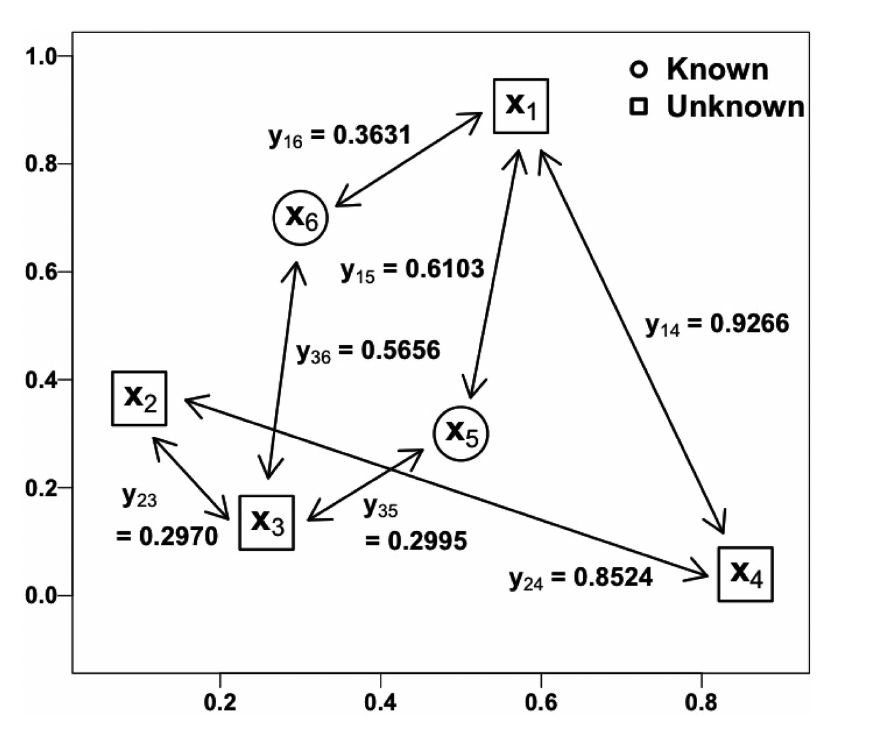
\includegraphics[width=\textwidth]{exa-3-sensor-plot.png}
    \caption{ The simulated distances $y_{ij} (= y_{ji} )$ among the six stationary sensor locations, $x_1 , x_2 , \ldots, x_6$, are displayed if observed.}
    \label{fig:exa3.0}
\end{figure}
\subsection*{Modified Problem}
We modify the setting of the problem a bit from original. We remove some locations and adjust observed distances to make a simpler
model. Although note that even with these simplifications the resulting posterior distributions have more complicated shapes.
We suppose there are six stationary sensors scattered
on a two dimensional space, and let $x_k^\top = (x_{k1}, x_{k2} )$ denote the
two-dimensional coordinates of the location of sensor k for
$k = 1, 2,\ldots,6.$ Now we assume that the locations of the last two
sensors, $x_5$ and $x_6$ , are known and the locations of the other
sensors, $x_1 , x_2, x_3 $, and $x_4$ are \textbf{unknown parameters of interest.}
The Euclidean distance between two sensors, $x_i$ and $x_j$ , denoted
by $y_{ij} (= y_{ji} )$, for $i = 1, 2, \ldots , 5$ and
$j = i + 1, \ldots , 6$. 
\paragraph{Likelihood:}We use the binary random variable to indicate whether this
observation(the
distance between $x_i$ and $x_j$) is available, i.e., if $y_{ij}$ is observed, it is one(1) and
otherwise it is zero. We denote this indicator variable by $w_{ij}(=w_{ji})$. It has the probability distributions for the observed data,
\begin{equation*}
    (w_{ij}|x_1,\ldots,x_4) \sim \text{Bernoulli}\left(exp\left(-\frac{||x_i-x_j||^2}{0.18}\right)\right)
\end{equation*}
The distance between two sensors is a random variable with noise(Gaussian measurement error). So the sensor $i$ has some distance from sensor $j$, and it has some probability distribution that is given by,
\begin{align*}
    (y_{ij}|w_{ij}=1,x_1,\ldots,x_4) \sim \mathcal{N}(||x_i-x_j||,\underbrace{0.02^2}_{noise})
\end{align*}
Now we can understand that $w_{ij}=1$, if we have some specified $y_{ij}$, between $i$ \& $j$, otherwise it is zero. So we can write the eight-dimensional likelihood
function,
\begin{multline*}
    L(x_1,x_2,x_3,x_4) \propto \prod_{j>i} \left[exp\left(-\frac{(y_{ij}-||x_i-x_j||)^2}{2x0.02^2}\right)\\
    \text{ x }exp\left(-\frac{w_{ij}x||x_i-x_j||^2}{2x0.03^2}\right)\text{ x }\left(1-exp\left(-\frac{||x_i-x_j||^2}{2x0.03^2}\right)\right)^{1-w_{ij}}\right]
\end{multline*}
\paragraph{Prior:}For each unknown location parameter, $x_1,\ldots,x_4$, we have a prior. The prior is assumed to be a diffuse bivariate Gaussian. It has mean $0,0)$, and covariance matrix $10^2$ x $I_d$. So, we write:
\begin{equation*}
    x_i \sim \mathcal{N}_2(x_4|\mathbf{0},10^2I_2)
\end{equation*}
\paragraph{Posterior:}As we now have our likelihood and prior, using Bayes rule we can write the full posterior distribution up to proportionality constant. It is,
\begin{equation*}
    f(x_1,x_2,x_3,x_4|y,w) \propto L(x_1,x_2,x_3,x_4) \text{ x }exp\left(-\frac{\sum_{i=1}^4 x_i^\top x_i}{2  \text{ x }10^2}\right)
\end{equation*}
here $y = \{y_{ij} , i > j\}$ and $w = \{w_{ij} , i > j\}$.
\texttt{Remark:} This model may
suffer from nonidentifiability when the number of observed
distances is small because unknown locations appear in the
likelihood only through distances; if $y_{ij}$ is observed between
an unknown $x_i$ and a known $x_j$ , the posterior distribution of $x_i$
may form a circle around $x_j$ without further observations.
\subsection*{Implementation}
It is evident that we don't have closed form for posterior distribution. We have to used approximation method like MCMC. We use Gibbs Sampler for sampling. It is done by iteratively sampling the four bivariate conditionals denoted by $$f_i (x_i | \{x_j , j \neq i\}, y, w) \text{  for } i = 1, 2, 3, 4.$$ Notice that none of these bivariate conditionals are a standard
distribution, from which we can sample directly using some computer software. So to sample from these, we use Metropolis or RAM kernels that are invariant with respect
to each conditional distribution. The paper have also used tempered transition, but we do not implement it. For our project purpose main algorithm is RAM but we also implement using Metropolis just to compare with RAM.
\subsubsection*{RAM within Gibbs Sampler}
To sample $x_i$ from a RAM kernel that is marginally invariant to $f_i(.)$ , we must
keep track of the auxiliary variable during the run, i.e., $\{z_i^{(k)}, k = 0, 1, 2,\ldots\}$. Why is that? \texttt{Reason:} Because $\{z_i^{(k)}, k = 0, 1, 2,\ldots\}$ are introduced solely to enable sampling $x_i$ from a RAM kernel, only $x_i^{(k)}$ is used to sample the other locations, and $z_i^{(k)}$ is used to draw $x_i^{(k+1)}$ at the next iteration.
\begin{tcolorbox}[colback=blue!5!white,colframe=blue,title=A RAM within Gibbs Sampler]
\begin{itemize}
    \item To sample $x_i$ can be given, at iteration $k$:
    \item Draw $y_i^{'} \sim q^D(y_i^{'}|x_i^{(k-1)})$.
    \item Draw $x_i^{*} \sim q^U(x_i^{*}|y_i^{'})$.
    \item Draw $z_i^{*} \sim q^D(z_i^{*}|x_i^{*})$.
    \item Set $(x_i^{(k)},z_i^{(k)})$ to $(x_i^{*},z_i^{*})$ with the probability $\alpha^J (x_i^{*},z_i^{*}|x_i^{(k-1)},z_i^{(k-1)})$, 
    Otherwise set $(x_i^{(k)},z_i^{(k)})$ to $(x_i^{(k-1)},z_i^{(k-1)})$.
\end{itemize}
\end{tcolorbox}
\subsection*{Results}
For comparing RAM with Gibbs and Metropolis within Gibbs, we have different lengths of each chain. First method of comparison is: the average number of evaluations of $f(.)$ ’s per iteration. The table 3 gives $N_{RAM}^{\pi}=37.72$ and $N_{M}^{\pi}=4$. It means the number of $f$'s evaluations in an iteration for RAM is much higher than Metropolis. Clearly $N_{RAM}^{\pi}=37.72$ indicates about nine density evaluations are required to sample each of the $f_i$’s. Also note that, RAM improves the acceptance rate of
Metropolis given the same jumping rule
without additional tuning. Although we have taken only 20000 samples with burn size to be 2000, due to computational restrictions, but bare in mind that these number are average numbers so they reflect approximately exact situation.
\begin{table}[H]
\caption{ The sampling results summarize $N_X^{\pi},(N_d,N_u,N_z)$, and Accept Rate for RAM and Metropolis} % title of Table
\centering % used for centering table
\begin{tabular}{c c c c } % centered columns (4 columns)
\hline\hline %inserts double horizontal lines
Kernel & $N_X^{\pi}$ & (N_d,N_u,N_z) &Accept-Rate  \\ [0.5ex] % inserts table
%heading
\hline % inserts single horizontal line
RAM & 37.72 & $x_1$:9.92(1,7.85,1.07) & 0.00295\\
 &  & $x_2$:9.07(1,7.00,1.07) & 0.00895\\
  &  & $x_3$:9.54(1,7.48,1.05) & 0.00355\\
   &  & $x_4$:9.17(1,7.04,1.12) & 0.00820\\% inserting body of the table
Metropolis & 4 & 1 for each $x_1,x_2,x_,x_4$ &0.00075\\
 &  &  & 0.00125\\
  &  &  & 0.00105\\
   &  &  & 0.00125\\[1ex] 
   % [1ex] adds vertical space
\hline %inserts single line
\end{tabular}
\label{table:nonlin} % is used to refer this table in the text
\end{table}
\paragraph{}The scatter plots(in figure ~\ref{fig:exa3.1}) of the posterior samples of each
unknown sensor location (columns) obtained by RAM and Metropolis(rows) are given. Note that in these plots, the dashed lines indicate the coordinates of the true location. Also observe that, the RAM sample is more dispersed than that
of Metropolis with the same jumping rule. It is specifically true for $x_1$ , $x_2$ , and $x_4$. From figure ~\ref{fig:exa3.2} we have the relative sizes of modes for the first
coordinate of each unknown location (columns) obtained by each
sampler (rows). The vertical dashed
lines indicate the true sensor locations. Clearly it is observable that, RAM represents all four
distributions and four sensors locations better than Metropolis does.
\texttt{Note:} Due to computational \textit{limitations} we sample only for 20000 samples. That is why our plots are not quite good to explain some of the things, but we believe that with more samples those things can be explained.
\begin{figure}[!htbp]
    \centering
    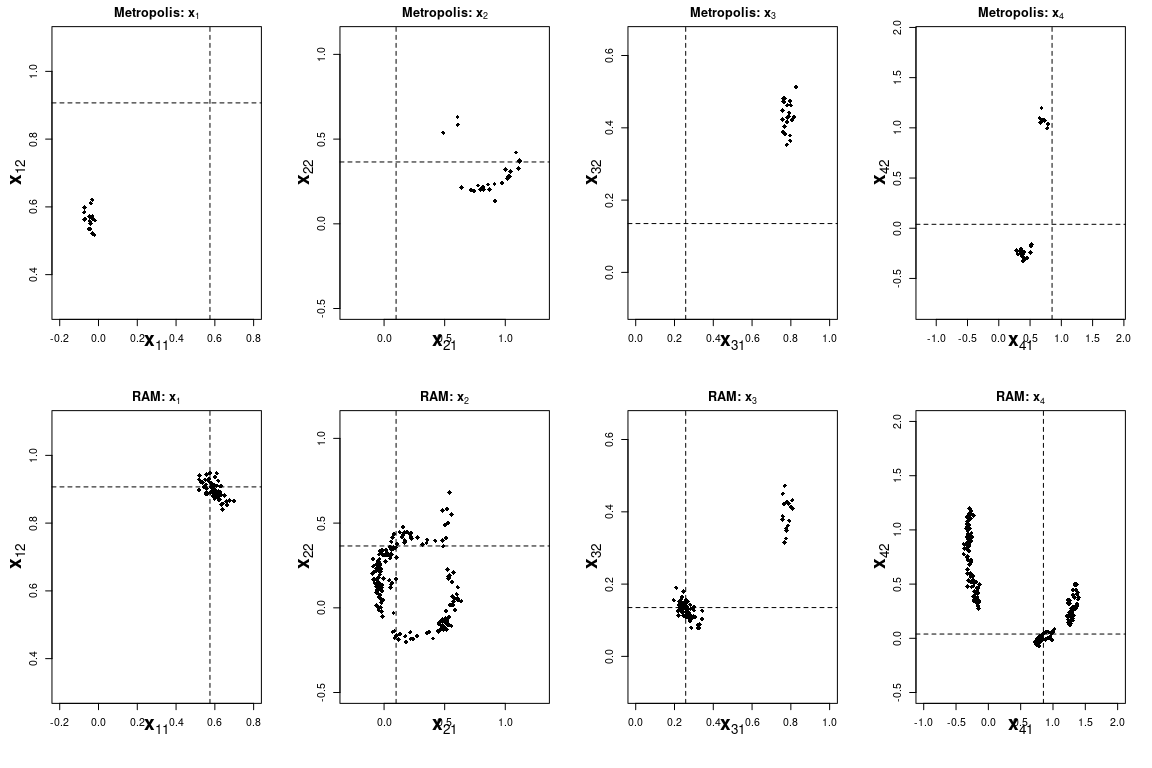
\includegraphics[width=\textwidth]{20000-3a-bold.png}
    \caption{Scatter plots of the posterior sample of each location (columns) obtained by different samplers (rows). The coordinates of the unknown sensors are denoted by
dashed lines}
    \label{fig:exa3.1}
\end{figure}
\begin{figure}[!htbp]
    \centering
    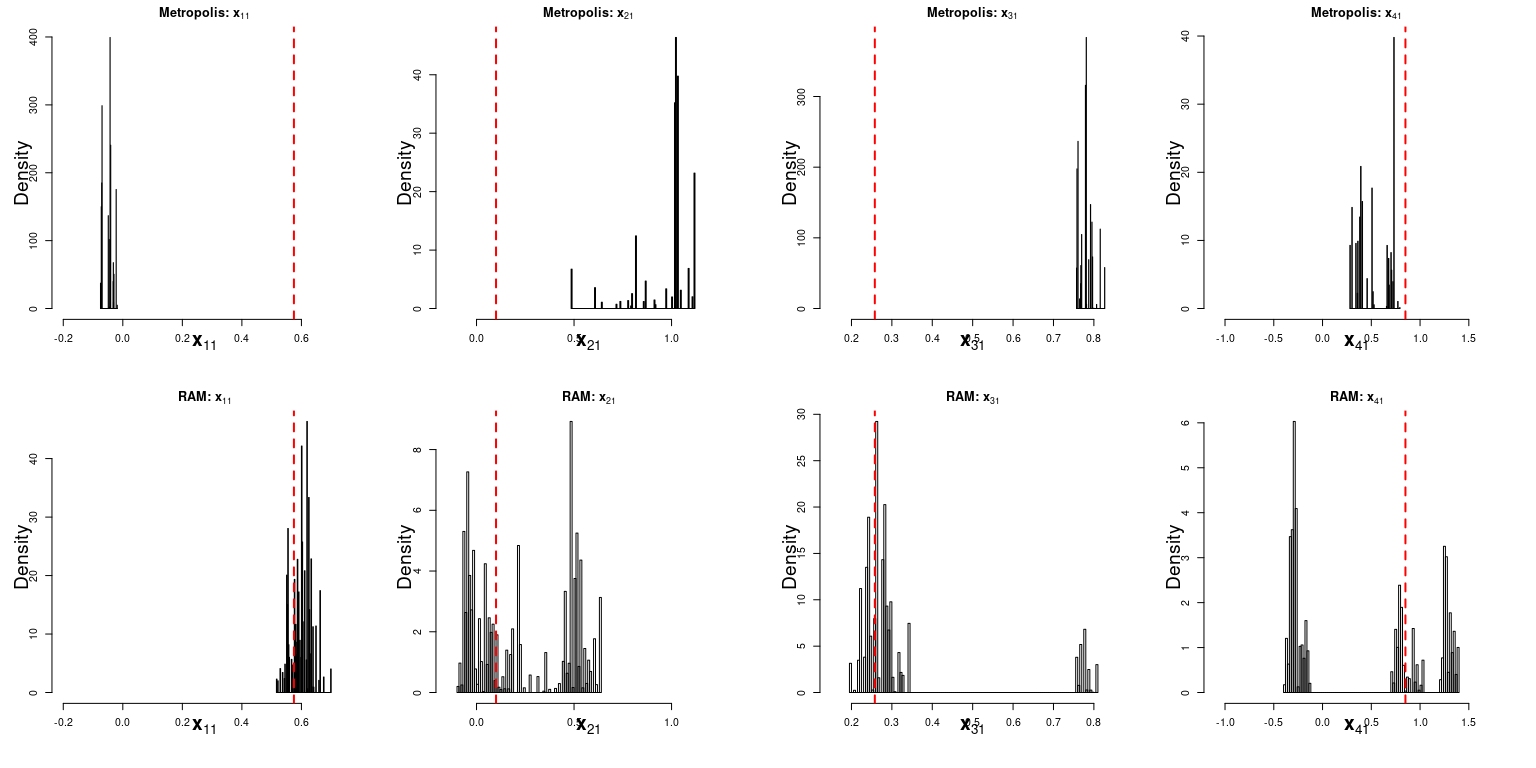
\includegraphics[width=\textwidth]{20000-3b-bold2.png}
    \caption{ Histograms of the posterior sample of each first coordinate (columns) obtained by different kernels (rows).}
    \label{fig:exa3.2}
\end{figure}
\clearpage
\subsection{Example 4: Strong Lens Time Delay Estimation
}
In this example we consider a applied astrophysical
problem that originally motivated Tak et. al.(2017) for the development of RAM algorithm. This problem gives rise to a multi modal target distribution, where one mode is extremely distant from the others. 
\subsection*{Physics Background}
Quasars are the most luminous active galaxies in the
Universe that host an accreting supermassive black hole at the center. The
path that light takes from a quasar to Earth can be altered by the gravitational field of a massive intervening galaxy, acting as a lens and bending
the trajectory of the emitted light. When the
quasar, lensing galaxy, and Earth are geometrically aligned, multiple images
of the quasar can appear in slightly different locations in the sky, from the
perspective of an observer on Earth. This phenomenon is known as strong
gravitational lensing. In this case, there are typically two or more
replicate images, referred to as doubly- or multiply-lensed quasars. Since
quasars are highly luminous, they can be seen at great distances, which
both enhances the possibility of lensing by an intervening galaxy and makes
them useful for cosmology.
The light rays forming each of these gravitationally lensed quasar images
take different routes from the quasar to Earth. Since both the lengths of the
pathways and the gravitational potentials they traverse differ, the resulting
multiple images are subject to differing lensing magnifications and their light
rays arrive at the observer at different times. Because of this, any fluctuations
in the source brightness are observed in each image at different times. From
a statistical perspective, we can construct a time series of the brightness of
each image, known as a light curve. Features in these \textit{light curves} appear to
be shifted in time and these shifts are called \textit{time delays}.
\begin{figure}[ht]
    \centering
    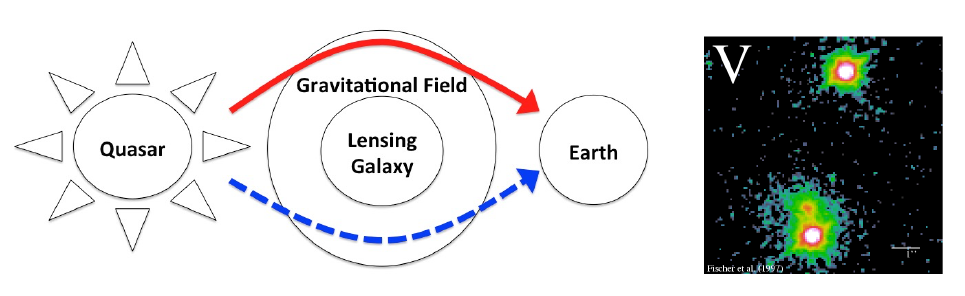
\includegraphics[width=\textwidth]{Screenshot from 2021-05-13 06-49-57.png}
    \caption{The gravitational field of an intervening galaxy acts as a lens deflecting two light
rays of a quasar image towards the Earth as shown in the left panel. An optical V-band image of the doubly-lensed quasar $Q0957+561$ obtained with the Canada France Hawaii telescope appears in the right panel. Figure have been taken from TAK ET AL.(2017)}
    \label{fig:my_label}
\end{figure}
\subsection*{Data}
We plot a pair of simulated light curves from
two irregularly observed time series of the
brightness of the doublylensed quasar $Q0957 + 561$ (Hainline
et al. 2012) in figure ~\ref{fig:exa4.0}; the light curves are labeled as A and B. \texttt{Note:} The brightness is reported on
the magnitude scale, an astronomical logarithmic measure of brightness, in
which smaller numbers correspond to brighter objects.
\begin{figure}
    \centering
    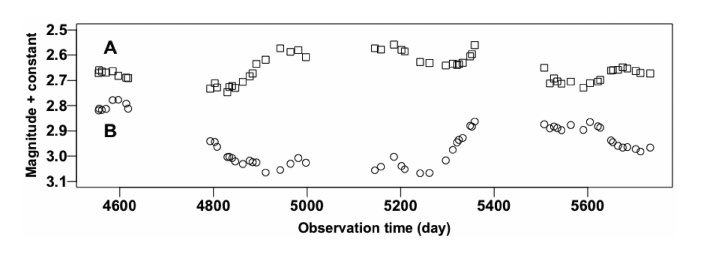
\includegraphics[width=\textwidth]{exa4-image.png}
    \caption{ Two observed time series of doublylensed quasar $Q0957 + 561$ (Hainline
et al. 2012). Time series A is denoted by squares and time series B is denoted by circles.}
    \label{fig:exa4.0}
\end{figure}
\paragraph{}For a doubly-lensed quasar, there are four variables recorded on an irregularly spaced sequence of observation times $\boldsymbol{t} = (t_1 , t_2, \ldots, t_n)^\top$ ; the observed
magnitudes $\boldsymbol{x} = (x_1 , x_2, \ldots , x_n )^\top$ for light curve A and $\boldsymbol{y} = (y_1 , y_2 , \ldots, y_n )^\top$
for light curve B as well as standard deviations, $\boldsymbol{\delta} = (\delta_1 , \delta_2, \ldots, \delta_n )^\top$ and
$\boldsymbol{\eta} = (\eta_1 , \eta_2 , \ldots , \eta_n)^\top$, representing their uncertainties due to heteroskedastic measurement error. There are
57 observations in each time series, that is, $n = 57$. Also note in ~\ref{fig:exa4.0} that both time series are plot-
ted with an offset (constant) in magnitude, but this does not affect the time delay
estimation. Since the time delay is estimated via relative comparison between fluctuations in the two light curves, our analysis is insensitive
to this overall additive constant.
\subsection*{Bayesian Model}
\subsubsection*{Latent time series}
We assume that each time-delayed light curve
is generated from a latent curve representing the true source magnitude in
continuous time. We denote these latent curves by $\mathbf{X} = \{X(t), t \in \mathbb{R}\}$
and $\mathbf{Y} = \{Y (t), t \in \mathbb{R}\}$, respectively, where $X(t)$ and $Y (t)$ are unobserved true magnitudes at time $t$. We use the vector notation $\mathbf{X(t)} =
(X(t_1 ), X(t_2), \ldots , X(t_n ))^\top$ and $\mathbf{X(t)} = (Y (t_1 ), Y (t_2 ), \ldots , Y (t_n ))^\top$ to denote
the n magnitudes of each latent light curve at the irregularly-spaced observation times $t$.
\paragraph{}We further assume that one of the latent brightness
curves is a shifted version of the other, that is,
\begin{equation*}
    Y(t_j)=X(t_j-\Delta)+\beta_0,
\end{equation*}
here $\Delta$ is the unknown time delay and $\beta_0$ is an unknown magnitude offset. The key
advantage of this model is that a single latent light curve, here X, is sufficient
to represent the true magnitude time series of the two (or more) lensed
images. Why is it a reasonable model? The curve-shifted model captures
the essential physical effects of strong gravitational lensing (at least in the
absence of microlensing), and thus is an appropriate model for estimating
the time delay.
\subsubsection*{Distribution of the observed data(Likelihood)}
Observing the gravitationally-
lensed images with a telescope, an astronomer measures the magnitude in
each image, $x_j$ and $y_j$ , and reports standard deviations, $\delta_j$ and $\eta_j$ , representing the uncertainties of the magnitudes due to measurement errors at time $\boldsymbol{t} = (t_1 , t_2, \ldots, t_n)^\top$. Note that these errors(the magnitude estimate and standard deviation) typically summarize a Gaussian approximation to the likelihood of the latent magnitude for the flux data of an image. Here, the observed magnitudes given the latent magnitudes are
assumed to be independent Gaussian variables with center at the latent magnitudes $X(t_j)$ and $Y (t_j )$, i.e.,
\begin{align*}
    x_j|X(t_j) & \sim \mathcal{N}(X(t_j),\delta_j^2)\\
    y_j|Y(t_j) & \sim \mathcal{N}(Y(t_j),\eta_j^2).
\end{align*}
Now, using shifted version model we can express the model for $y_j$ as,
\begin{equation*}
    y_j|(X(t_j-\Delta),\Delta,\beta_0) \sim \mathcal{N}(X(t_j-\Delta)+\beta_0,\eta_j^2).
\end{equation*}
Given $\Delta$, we define $\boldsymbol{t}^{\Delta} = (t_1^{\Delta},\ldots,t_2n^{\Delta})^\top$
 as the sorted vector of $2n$ times
among the $n$ observation times, $\boldsymbol{t}$, and the $n$ time-delay-shifted observation
times, $\boldsymbol{t} - \Delta$. Also, $\mathbf{X}(\boldsymbol{t}^{\Delta}) = (X(t_1^{\Delta}),\ldots, X(t_2n^{\Delta}))^\top$
 is the vector of
$2n$ latent magnitudes at the times in $t^{\Delta}$
. The joint density function of the
observed data given $\mathbf{X}(\boldsymbol{t}^{\Delta}), \Delta,$ and $\boldsymbol{\beta}$ is,
\begin{equation*}
    p(\boldsymbol{x},\boldsymbol{y}|\mathbf{X}(\boldsymbol{t}^{\Delta}), \Delta,\boldsymbol{\beta}) \propto \prod_{n=1}^N \left[p(x_j|X(t_j)) \text{ x } p(y_j|(X(t_j-\Delta),\Delta,\boldsymbol{\beta}))\right]
\end{equation*}
\subsubsection*{Prior distributions}
We assume $X (.)$ follows an Ornstein–Uhlenbeck process
(Kelly, Bechtold, and Siemiginowska 2009). The stochastic differential equation,
\begin{equation*}
    dX(t)=-\frac{1}{\tau}(X(t)-\mu)dt+\sigma dB(t).
\end{equation*}
Solving the above stochastic differential equation yields the sampling distribution of $X(t^{\Delta})$, where $\boldsymbol{t}^{\Delta} = (t_1^{\Delta},\ldots,t_2n^{\Delta})^\top$ contains the sorted $2n$
times among the $n$ observation times, $t$, and the $n$ time-delay-
shifted observation times,$\boldsymbol{t} - \Delta$. Specifically,
\begin{equation*}
    X(t_1^{\Delta})|(\Delta,\theta) \sim \mathcal{N}_1(\mu,\frac{\tau \phi^2}{2}),
\end{equation*}
and for $j = 2, 3, \ldots , 2n$,
\begin{equation*}
    X(t_j^{\Delta})|(X(t_{j-1}^{\Delta}),\delta,\theta) \sim \mathcal{N}_1(\mu+a_j(X(t_{j-1}^{\Delta})-\mu)),\frac{\tau \phi^2}{2}(1-a_j^2))
\end{equation*}
Here $\theta=(\mu,\phi^2,\tau)^\top$ and  $a_j=exp\left(-\frac{(t_j^{\Delta}-t_{j-1}^{\Delta})}{\tau}\right)$ that is a shrinkage factor that depends on the
observational cadence and $\tau$. Hence the joint prior density function of the $2n$ latent magnitudes is,
\begin{equation*}
    p(\mathbf{X}(\boldsymbol{t}^{\Delta})|\Delta,\theta) = p(X(t_1^{\Delta})|\Delta,\theta) \text{ x } \prod_{j=2}^{2n} p(X(t_j^{\Delta})|X(t_{j-1}^{\Delta}),\delta,\theta)
\end{equation*}
In the paper authors have followed Tak et al. (2017) to set the model parameter priors. We do the same and, we set \texttt{independent priors} for the model parameters:
\begin{align*}
    \Delta & \sim Uniform[−1178.939, 1178.939],\\
    \beta_0 & \sim Uniform[−60, 60],\\
    \mu & \sim Uniform[−30, 30],\\
    \phi^2 & \sim inverse-Gamma(1, 2/10^7 ),\\
    \tau & \sim inverse-Gamma(1, 1).
\end{align*}
\subsubsection*{Posterior Distribution}
It is quite evident that we are not going to get a closed form expression for posterior distribution. We do get posterior distribution up to proportionality constant and it is,
\begin{multline*}
    f(\mathbf{X}(\boldsymbol{t}^{\Delta}),\theta,\Delta,\boldsymbol{\beta}|\boldsymbol{x},\boldsymbol{y}) \propto \left[\prod_{n=1}^N p(x_j|X(t_j)) \text{ x } p(y_j|(X(t_j-\Delta),\Delta,\boldsymbol{\beta}))\right] \\ \text{ x } \left[p(X(t_1^{\Delta})|\Delta,\theta) \text{ x } \prod_{j=2}^{2n} p(X(t_j^{\Delta})|X(t_{j-1}^{\Delta}),\delta,\theta)\right] \text{ x } h(\theta,\Delta,\beta_0)
\end{multline*}
Here $h(\theta,\Delta,\beta_0)$ is simply product of all the model parameter priors as they all are independent from each other.
\subsection*{Sampling}
Now, since posterior distribution does not have a closed form, we have to use approximation method like MCMC. Here we use Gibbs Sampler, wherever we don't have closed form for Conditional Posteriors for Gibbs, we use other MCMC techniques like RAM, MH, and, MH with a mixture proposal distribution. Specifically, since we cannot
directly sample $p( \Delta| \beta_0 , \theta )$ in Step 1 and the marginal posterior distribution of is often multi modal, we use these MCMC algorithms. Overall Gibbs Sampler depends on which algorithm we use in Step-1 to sample from $p( \Delta| \beta_0 , \theta )$.
\begin{tcolorbox}[colback=blue!5!white,colframe=blue,title=A Metropolis-Hastings within Gibbs Sampler]
\begin{itemize}
    \item \texttt{Initialization:} Set $\Delta^{(0)} , \mathbf{X}^{(0)} (\boldsymbol{t}^{\Delta^{(0)}}
 ), \beta_0^{(0)}$ , and $\theta^{(0)}$ . For $i = 1, 2, \ldots ,$
    \item \texttt{Step-1:} Draw $(\mathbf{X}^{(i)} (\boldsymbol{t}^{\Delta^{(i)}}
 ),\Delta^{(i)}) \sim p(\mathbf{X} (\boldsymbol{t}^{\Delta}
 ),\Delta|\beta_0^{(i-1)},\theta^{(i-1)})$\\$=p_1(\Delta|\beta_0^{(i-1)},\theta^{(i-1)})p_2(\mathbf{X} (\boldsymbol{t}^{\Delta}
 )|\Delta,\beta_0^{(i-1)},\theta^{(i-1)})$.
    \item \texttt{Step-2:} Draw $\beta_0^{(i)} \sim p(\beta_0|\mathbf{X}^{(i)} (\boldsymbol{t}^{\Delta^{(i)}}
 ),\Delta^{(i)}),\theta^{(i-1)})$,
 \item \texttt{Step-3:} Draw $\theta^{(i)} \sim p(\theta|\beta_0|\mathbf{X}^{(i)} (\boldsymbol{t}^{\Delta^{(i)}}
 ),\Delta^{(i)}),\beta_0^{(i)})$.
\end{itemize}
\end{tcolorbox}
\subsubsection*{RAM in Step-1}
The mixture jumping rule
generates a proposal from the Gaussian jumping rule used by
Metropolis with probability 0.5 and from the prior distribution of $\Delta$ otherwise. To sample $\Delta$ using the RAM kernel, we
additionally keep track of the auxiliary variable during the run,
that is, $\{z_i^{(k)}, k = 0, 1, 2,\ldots\}$. Why is that? \texttt{Reason:} Because $\{z_i^{(k)}, k = 0, 1, 2,\ldots\}$ are
introduced solely to enable sampling $\Delta$ from the RAM kernel,
only $\Delta^{(i)}$ is used to sample $\mathbf{X}(\boldsymbol{t}^{\Delta}),\theta$, and $\beta_0$ in the other steps, and $z^{(i)}$ is used to draw $\Delta^{(i+1)}$ at the next iteration. 
At iteration $i$, we sequentially draw $\Delta^{'} \sim q^D(\Delta^{'}|\Delta^{(i-1)}), \Delta^{* } \sim q^U(\Delta^{*}|\Delta^{'})$, and, $z^{*} \sim q^D(z^{*}|\Delta^{*})$. We set $(\Delta^{(i)},z^{(i)})$ to $(\Delta^{*},z^{*})$ with acceptance probability $\alpha^J((\Delta^{*},z^{*})|(\Delta^{(i-1)},z^{(i-1)}))$, and set $(\Delta^{(i)},z^{(i)})$ to $(\Delta^{(i-1)},z^{(i-1)})$ otherwise.
\paragraph{}
In above MHwG algorithm \textbf{initialization} is important and we set initial values following the paper. We also can observe that multiple initial values
spread across the entire range will result in nearly identical posterior distributions. In all these cases, we set $q$ to be Gaussian with $\sigma = 700$. Initialization,
\begin{itemize}
    \item for $\Delta$, initiating at the center of the
entire range of $\Delta$, that is, $\Delta^{(0)}=0$.
\item $\phi^{(0)}=0.01,\tau^{(0)}=200,\mu^{(0)}=\frac{\sum_{j=1}^n x_j  }{n}=2.658,\beta_0^{(0)}=\frac{\sum_{j=1}^n (y_j-x_j)}{n}=-0.113$.
\item $\mathbf{X}^{(0)} (\boldsymbol{t}^{\Delta^{(0)}}
 )$ is  a vector of $\boldsymbol{x}$ and $\boldsymbol{y}-\beta_0^{(0)}$  that are sorted
in time, $\boldsymbol{t}$ for $\boldsymbol{x}$ and $\boldsymbol{t}-\Delta$ for $\boldsymbol{y}-\beta_0^{(0)}$. 
\end{itemize}
\subsection*{Results}
We use, the total number of jumps
between the two distant modes in the post burn-in sample,
denoted by $N_{jumps}$, as our first measure to compare three algorithms used in Step-1. Notice in the table that, both versions of Metropolis have smaller number of jumps between modes than RAM. The RAM to Metropolis(both) ratio is about \textbf{1.7}. Also notice that RAM's acceptance rate is at least \textbf{3.25} times higher than both versions of Metropolis. Keep in mind that here we have assumed all three algorithms have same proposal distribution and no extra tuning have been done.

\begin{table}[H]
\caption{The sampling results summarize acceptance rate for $\Delta$, and $N_{jumps}$ for three kernels} % title of Table
\centering % used for centering table
\begin{tabular}{c c c } % centered columns (4 columns)
\hline\hline %inserts double horizontal lines
Kernel & $N_{jumps}$ & Accept-Rate  \\ [0.5ex] % inserts table
%heading
\hline % inserts single horizontal line
RAM & 326 & 0.052\\
Metropolis & 144 &0.016\\
Metropolis with mixture jumping rule & 190 &0.013\\
\hline %inserts single line
\end{tabular}
\label{table:nonlin} % is used to refer this table in the text
\end{table}
Figure ~\ref{fig:exa4.1} displays histograms of the posterior sample of
 obtained using the three different kernels.
The size of the mode near 423 days, which is of great scientific
interest, differs substantially among the samplers. In Figure ~\ref{fig:exa4.2}, we magnify this mode, superimposing a
curve that represents the marginal posterior density of based
on .18M posterior samples obtained with an oracle
sampler constructed with knowledge of both mode locations.
The size and shape of the mode near 423 days obtained with
RAM match the oracle sampler better than the other algorithms,
which is an algorithmic confirmation of the reliability of RAM. \texttt{Note:} Due to computational limitations we have taken .2M samples for RAM, .4M for MH, and, .6M for MH with mixture jumping rule.
\begin{figure}[!htbp]
    \centering
    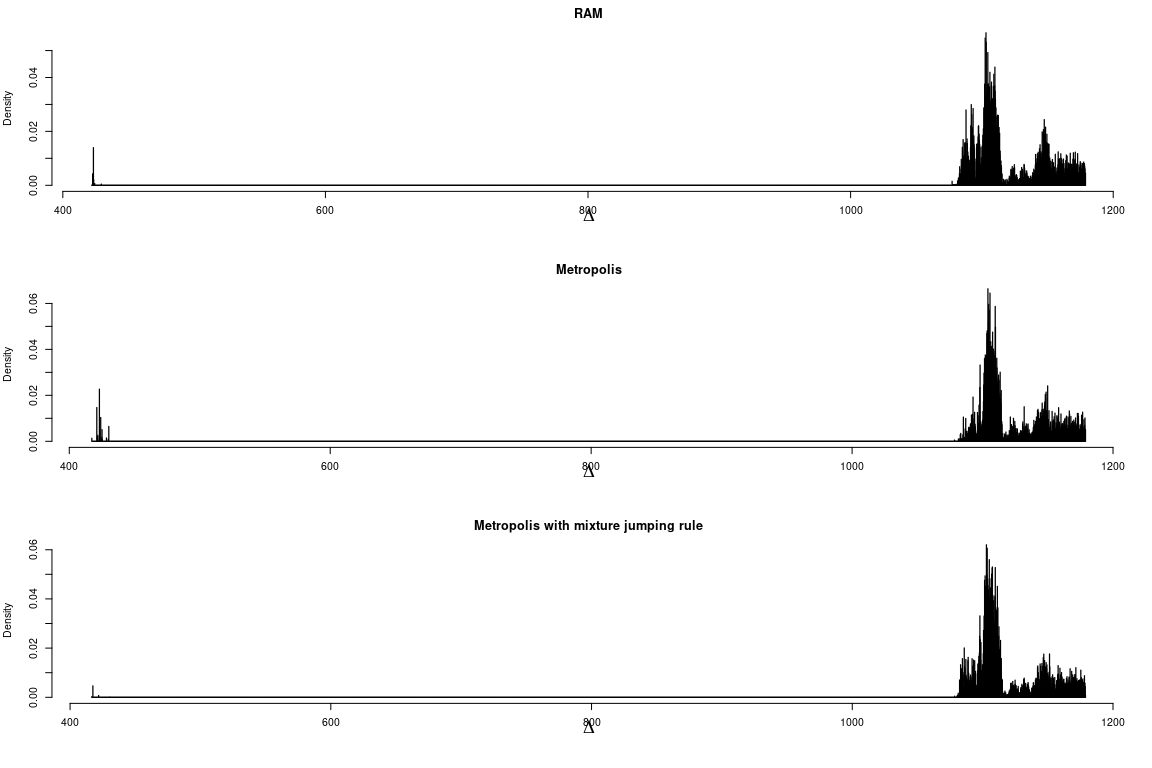
\includegraphics[width=\textwidth]{2-4-6(4a).png}
    \caption{The histograms based on the
posterior sample of $\Delta$}
    \label{fig:exa4.1}
\end{figure}
\begin{figure}[!htbp]
    \centering
    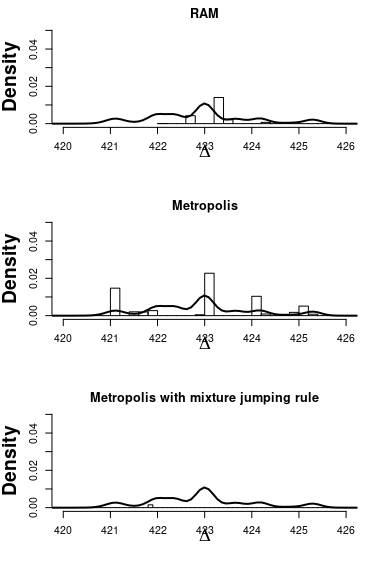
\includegraphics[,height=4in,width=0.8\textwidth]{image.png}
    \caption{The mode near 423 days and superimpose the posterior density of $\Delta$ obtained by an oracle sampler}
    \label{fig:exa4.2}
\end{figure}
\clearpage
\section{Concluding Remarks}
In this project RAM algorithm is being introduced as an alternative to deal with multi modality. With MH algorithm it is quite difficult to jump between multiple modes. This project also given some newer strategies of forming acceptance probabilities. More work is possible on this project. We can try to compare the theoretical convergence rate of
our algorithm to others, but this is difficult partially owing to the
intractable down-up jumping density, $q^{DU}$.
Also,for tuning RAM in various multi modal cases a better set of
strategies can be investigated. Another avenue for
further improvement is to apply the ideas of the mode-jumping
proposal and the delayed rejection method to RAM, e.g., allowing an asymmetric density function $q$ so that the downhill move
encourages longer jumps than the uphill move does.

\clearpage

\section*{\texttt{References}}
\small
\begin{enumerate}
    \item Kou, S. C., Zhou, Q., and Wong, W. H. (2006), “Discussion Paper:
Equi-Energy Sampler with Applications in Statistical Inference and
Statistical Mechanics,” The Annals of Statistics, 34, 1581–1619.
[479,482,483,484]
\item Tak, H., Mandel, K., van Dyk, D. A., Kashyap, V. L., Meng, X.-L., and
Siemiginowska, A. (2017), “Bayesian Estimates of Astronomical Time
Delays between Gravitationally Lensed Stochastic Light Curves,” The
Annals of Applied Statistics, 11, 1309–1348. [487,488]
\item Kelly, B. C., Bechtold, J., and Siemiginowska, A. (2009), “Are the Variations
in Quasar Optical Flux Driven by Thermal Fluctuations?” The Astro-
physical Journal, 698, 895–910. [488]
\item Hainline, L. J., Morgan, C. W., Beach, J. N., Kochanek, C., Harris, H. C.,
Tilleman, T., Fadely, R., Falco, E. E., and Le, T. X. (2012), “A New
Microlensing Event in the Doubly Imaged Quasar Q0957+561,” The
Astrophysical Journal, 744, 104–113. [487]
\item Møller, J., Pettitt, A. N., Reeves, R., and Berthelsen, K. K. (2006),
“An Efficient Markov Chain Monte Carlo Method for Distributions
with Intractable Normalising Constants,” Biometrika, 93, 451–458.
[479,481,482]
\end{enumerate}
\clearpage
\begin{appendix}
  \listoffigures
  \listoftables
\end{appendix}
\end{document}